% Base template source: https://tex.stackexchange.com/questions/8827/preparing-cheat-sheets

\documentclass{article}

\usepackage{multicol}
\usepackage{lipsum}

\setlength{\columnseprule}{0.4pt}

\usepackage{calc, ifthen,hyperref, gensymb, comment, textcomp}

\usepackage{amsmath,amsthm,amsfonts,amssymb}

\usepackage{color,graphicx,overpic}

\usepackage{geometry}
% This sets page margins to .5 inch if using letter paper, and to 1cm
% if using A4 paper. (This probably isn't strictly necessary.)
% If using another size paper, use default 1cm margins.
\ifthenelse{\lengthtest { \paperwidth = 11in}}
    { \geometry{top=.25in,left=.25in,right=.25in,bottom=.25in} }
    {\ifthenelse{ \lengthtest{ \paperwidth = 297mm}}
        {\geometry{top=1cm,left=1cm,right=1cm,bottom=1cm} }
        {\geometry{top=1cm,left=1cm,right=1cm,bottom=1cm} }
    }

% Turn off header and footer
\pagestyle{empty}

% Don't print section numbers
\setcounter{secnumdepth}{0}

% Define Image
\newenvironment{Figure}
     {\par\medskip\noindent\minipage{\linewidth}}
     {\endminipage\par\medskip}

% -----------------------------------------------------------------------

\begin{document}
\raggedright
\footnotesize

% Area Above Columns
\begin{center}
     \Large{\underline{Thermodynamics - Zak Olech - 9/10/2019}}
\end{center}

\begin{multicols}{3}

% multicol parameters
% These lengths are set only within the two main columns
%\setlength{\columnseprule}{0.25pt}
\setlength{\premulticols}{1pt}
\setlength{\postmulticols}{1pt}
\setlength{\multicolsep}{1pt}
\setlength{\columnsep}{2pt}



\section{Chapter 9}
\subsection{Air-Standard Otto cycle}
\lipsum[1]
\begin{Figure}
    \centering
    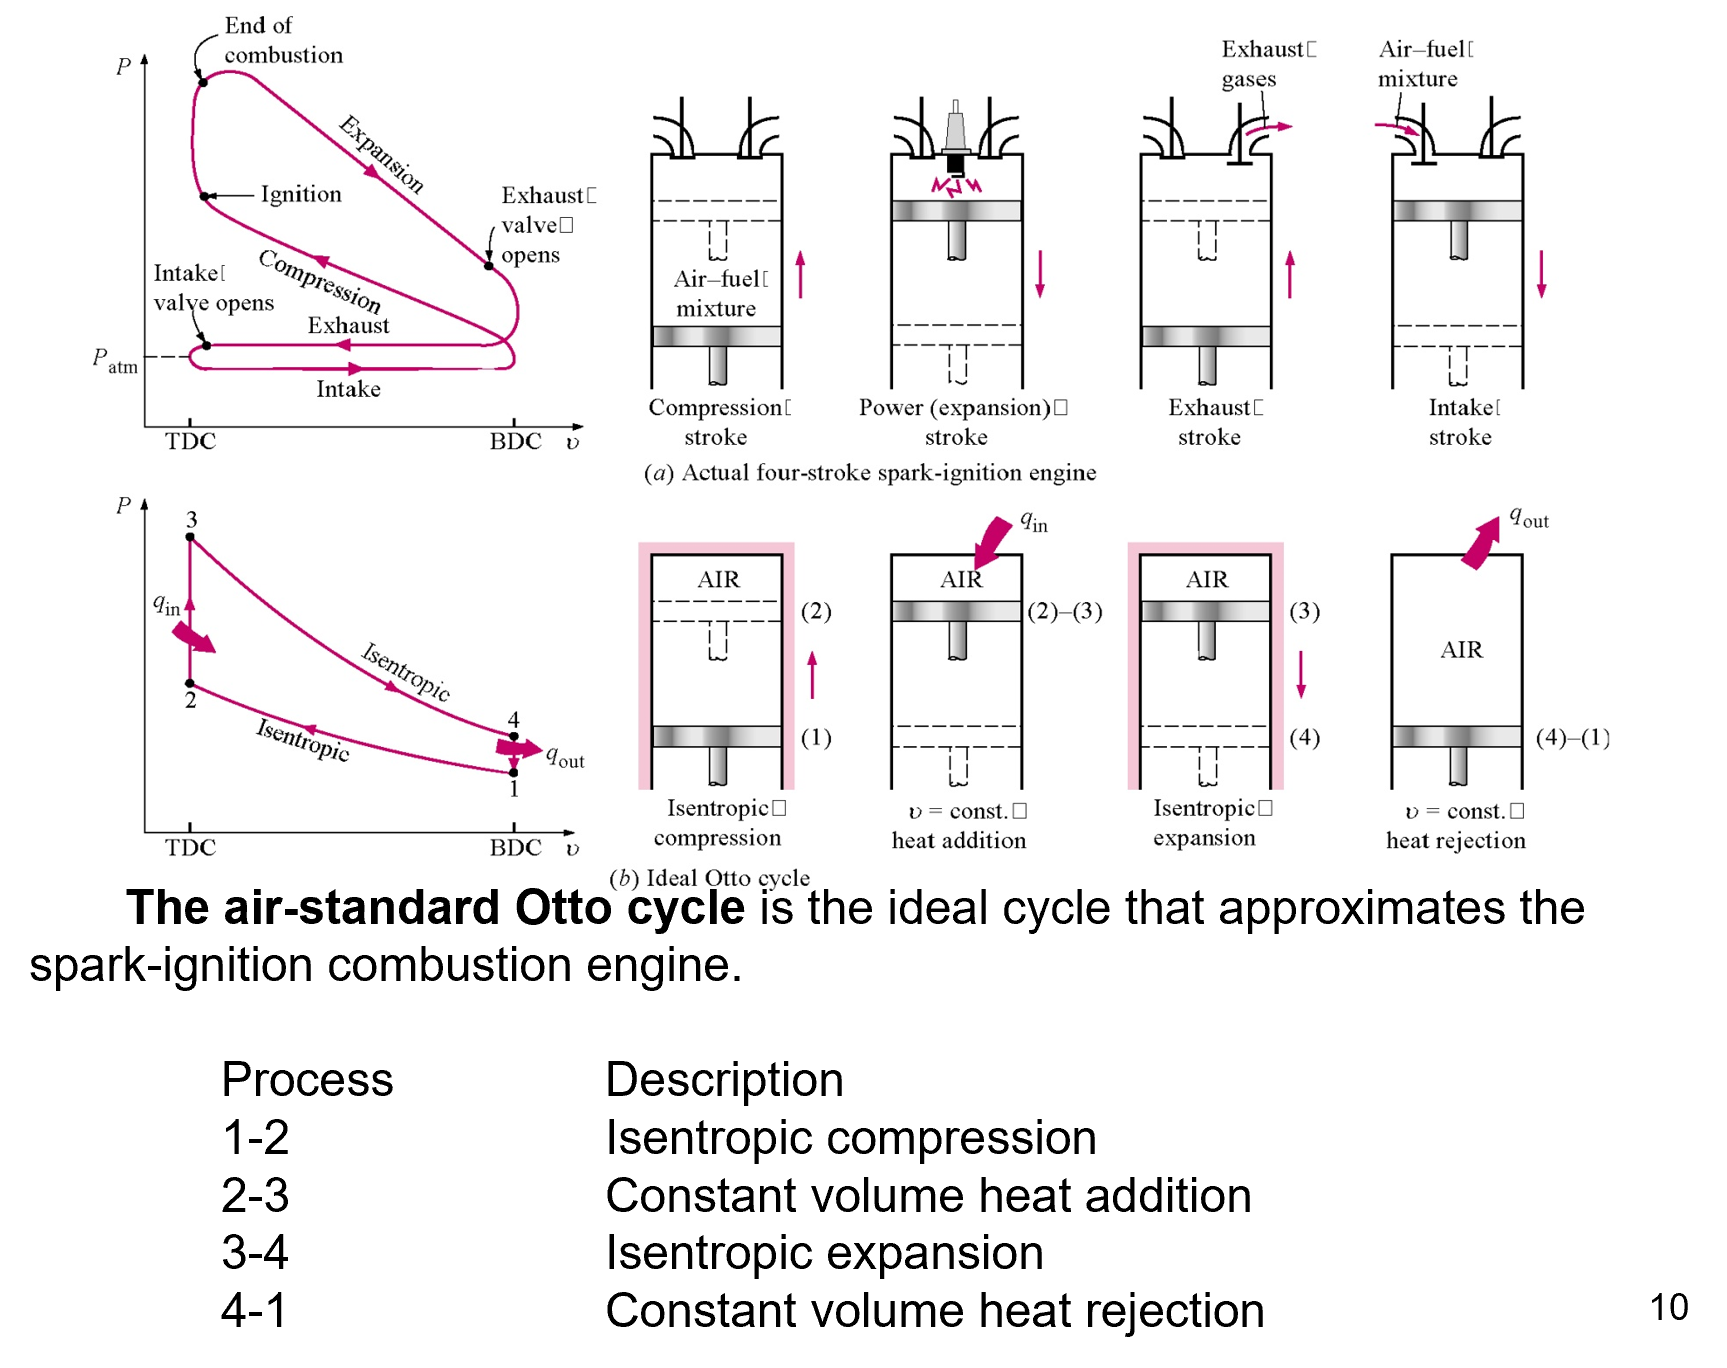
\includegraphics[width=\linewidth]{Air-Standard_OttoCycle.png}
\end{Figure}

\end{multicols}
\end{document}